\chapter{Optimizing SNSPD HBT and TCSPC measurement of a fs pulsed source}
In this chapter will be presented the procedures carried out to optimize the HBT and TCSPC measurements that we took with a femtosecond pulsed laser source.
In detail, \autoref{cpp:Motivations} provides the reader the driving motivations as well as a description of the experimental setup we used.
Moving forward with the structure of the chapter, \autoref{cpp:Initial-khaos} provides conditions, observations and conclusions behind the first chaotic measurement obtained with this setting.
Lastly, \autoref{cpp:Improvements&discussion} brings to the discussion the driving idea behind the troubleshooting, together with a qualitative discussion of the results obtained after such changes.



\section{Motivations and experimental setup overview}
\label{cpp:Motivations}
When studying pulsed laser light with the use of an SNSPD as a detector, it is good practice to question the results obtained with respect to the various jitter sources involved. Isolating such timing jitter sources can be a difficult task. For this reason a good approach can involve changing the pulsed laser light to another whose jitter is known, or also negligible under certain circumstances. By choosing this approach we substantially simplify the recognition of all the other jitter sources involved outside of the pulse generation jitter, providing an optimal setup to quantify the precision of the detection instrument. 
In this second part of this thesis we will then present the procedures of optimization that we carried out on HBT and TCSPC measurements obtained with a femtosecond pulsed laser, whose intrinsic jitter can easily be considered negligible when compared to the laser source of the first part.

In particular, the laser source we used is a mode-locked Titanium-Sapphire (Ti:Sa) laser, driven by a 6.34~W Sprout-G-15W laser manufactured by Lighthouse Photonics. Under these working conditions the Ti:Sa is capable of producing $\leq 100$~fs pulses. An important remark needs to be made about this temporal duration : although the manufacturer specifies that with a 5~W pump laser the output pulses can reach $\sim 50$~fs, these values correspond to nearly transform-limited pulses under optimal cavity alignment and dispersion compensation. In our case the output was not transform-limited, so we treated the Ti:Sa as a black box. The only verification we carried out on this black box relied on the real time spectrum of the laser. From the spectral measurement we were able to identify the operating wavelength, the spectral width and above all confirm the pulsed regime. In the case of a spectrum without a distinct peak, we would have concluded that the Ti:Sa was producing CW output instead of the desired pulsed regime.

The key differences with respect to the experimental setup presented in \autoref{sec:Overview} can be summarized as follows:
\begin{itemize}
    \item Ti:Sa femtosecond pulses replacing the previous EOM-driven source,
    \item Single-mode fiber (Thorlabs 780HP) instead of the polarization-maintaining fiber,
    \item TCSPC operated with a divided SYNC provided by a multifunctional divider box, yielding an effective frequency at the ID1000 of about 20~MHz.
\end{itemize}

An overview of the experimental setup can be found in \autoref{TisaSetup}.

\begin{figure}[hbtp]
\centering
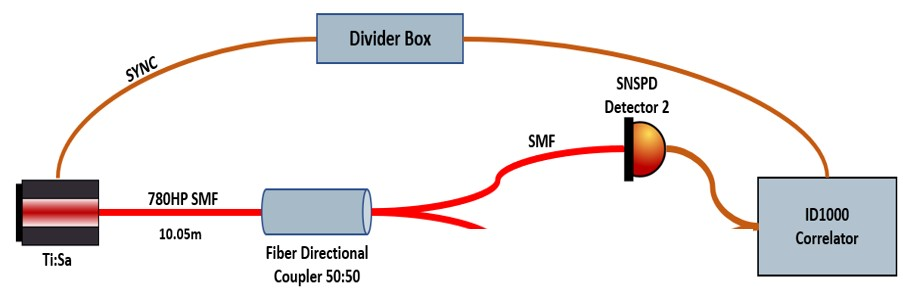
\includegraphics[width=1\textwidth]{TiSa_Setup.jpg}
\caption{Visual representation of the experimental setup. The pulsed output of the Ti:Sa laser (left) propagates through $\approx 10$~m of single-mode fiber (SMF) before reaching a fiber directional coupler. The beam is then divided into two channels that are directed to separate inputs of the SNSPD. Detection events are collected by the ID1000 time-tagger. Also shown are the electronic cables linking the Ti:Sa electronic pulser to the ID1000 via a multifunctional divider box.}
\label{TisaSetup}
\end{figure}




\section{Unwanted Side Peaks in HBT and TCSPC measurements}
\label{cpp:Initial-khaos}
At a regime of 3~MHz we ran the first set of measurements, over a time of 15s of exposure time.
The resulting histograms are then post-processed to shift the main peak in the zero time position, in order to ease the comparison between the different peaks.
\autoref{Khaos} shows the chaotic situation we got with the first measurement. So many side peaks appear, and the situation is far to be understood.

\begin{figure}[hbtp]
\centering
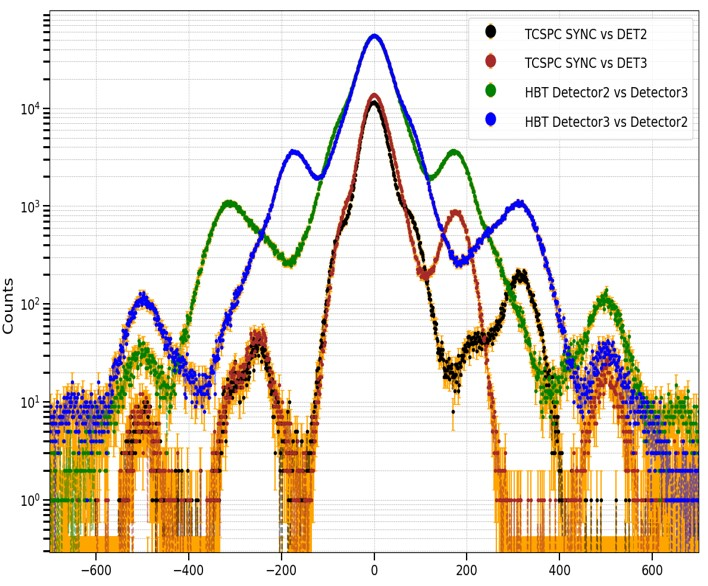
\includegraphics[width=1\textwidth]{Khaos.jpg}
\caption{Ciaone}
\label{Khaos}
\end{figure}

\section{Partly retrieving side peaks in HBT from coordinates of TCSPC peaks}
\label{cpp:Reconstructsides}

\begin{figure}[hbtp]
\centering
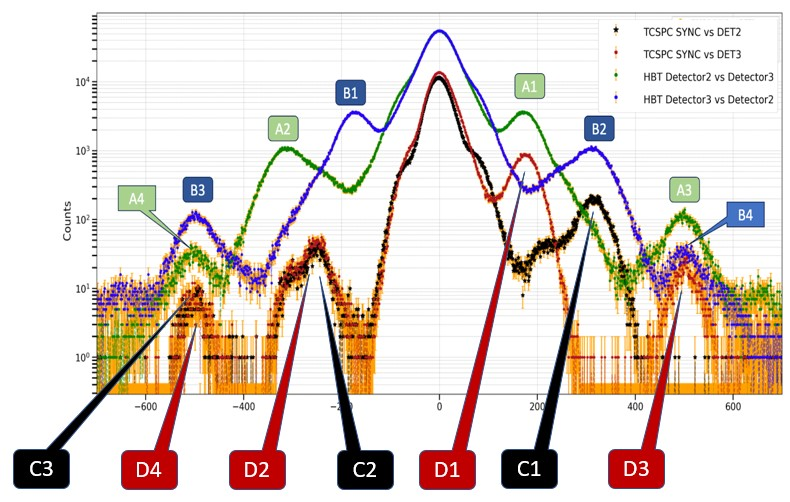
\includegraphics[width=1\textwidth]{Khaos_Labeled.jpg}
\caption{Ciaone}
\label{Khaos_labeled}
\end{figure}


\begin{table}[h!]
\centering
\caption*{\textbf{Detected position of the peaks}}
\renewcommand{\arraystretch}{1.3}
\begin{tabular}{
>{\centering\arraybackslash}m{1.5cm} 
>{\centering\arraybackslash}m{1.5cm} 
>{\centering\arraybackslash}m{1.5cm} 
>{\centering\arraybackslash}m{1.5cm} 
>{\centering\arraybackslash}m{1.5cm}}
\rowcolor{blue!50}
\textcolor{white}{\small[\textbf{ps}]} & \textcolor{white}{\textbf{A}} & \textcolor{white}{\textbf{B}} & \textcolor{white}{\textbf{C}} & \textcolor{white}{\textbf{D}} \\
\rowcolor{white}
\cellcolor{blue!50} \textcolor{white}{\textbf{0}} & 0    & 0    & 0     & 0     \\
\rowcolor{white}
\cellcolor{blue!50} \textcolor{white}{\textbf{1}} & 174  & -174 & 316   & 175   \\
\rowcolor{white}
\cellcolor{blue!50} \textcolor{white}{\textbf{2}} & -313 & 312  & -250  & -246  \\
\rowcolor{white}
\cellcolor{blue!50} \textcolor{white}{\textbf{3}} & 495  & -494 & -500  & +501  \\
\rowcolor{white}
\cellcolor{blue!50} \textcolor{white}{\textbf{4}} & -502 & 503  & n.d.  & -500  \\
\rowcolor{white}
\end{tabular}
\end{table}









\section{Measurements with improved detection thresholds}
\label{cpp:Improvements&discussion}

\subsection{Driving idea}
we strongly suspect that the chaotic behavior that we're getting, although we're visualizing the data always in log scale finds its origin in a sort of miscalibration of the triggering thresholds.
For this reason we managed to shut the laser and while the detector was receiving only stray photons, we looked at the electronic pulses coming out of the SNSPD.
Subsequently we initialized the Oscilloscope to visualize also the first derivative of the pulse so that we could get an info on where to locate the new, and refined threshold. The whole idea was to choose the point where the electrical signal expressed the greatest steepness, in order to achieve better measurements.
The whole idea we formulated explained the side peaks, as a consequence of having the detector measuring clicks when it was not fully recovered from the previous detection. By Modifying for a stronger threshold, as seen in \autoref{TrickShot}, we are getting rid of the even slow possibility to trigger with a non fully recovered nanowire.
Important mention is related to how we looked at these signals : instead of plugging the cable from the SNSPD straight into the Oscilloscope, we managed to add an impedence load to it, valued $50 \Omega$, to simulate the impedence that it will encounter at the entrance of the ID1000 Time-Tagger.

\begin{figure}[hbtp]
\centering
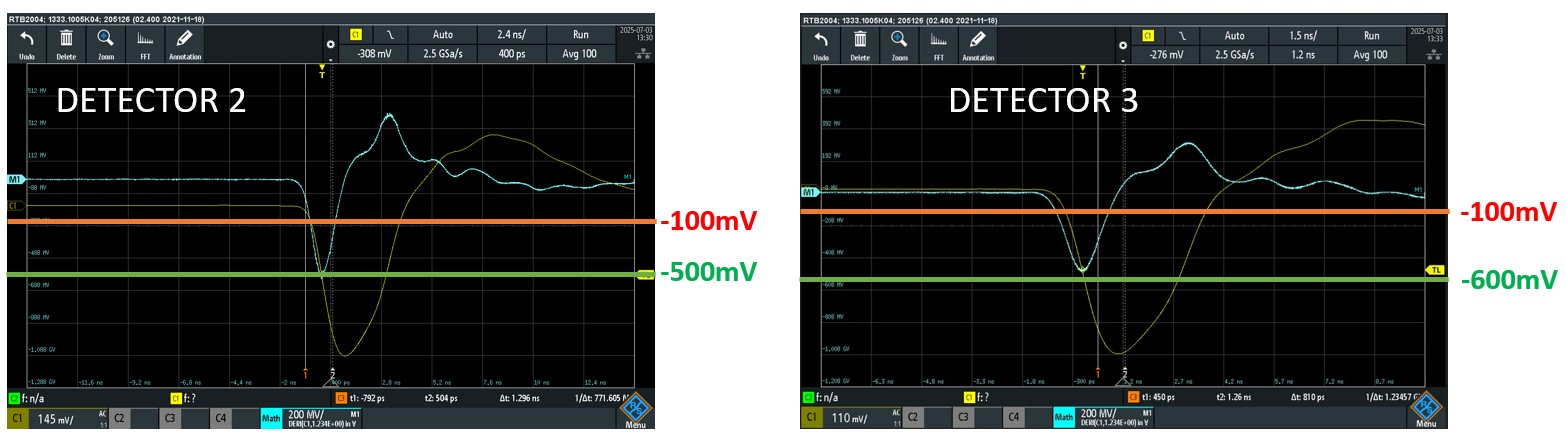
\includegraphics[width=1\textwidth]{ScopeShots.jpg}
\caption{Ciaone}
\label{TrickShot}
\end{figure}

As seen in \autoref{TrickShot}, by looking at the images we significantly modified the thresholds, passing from a value of $-100mV$ for both the detectors to $-500mV$ and $-600mV$, for detector 2 and detector 3 respectively.

\subsection{Discussion of the new measurements}
\begin{figure}[hbtp]
\centering
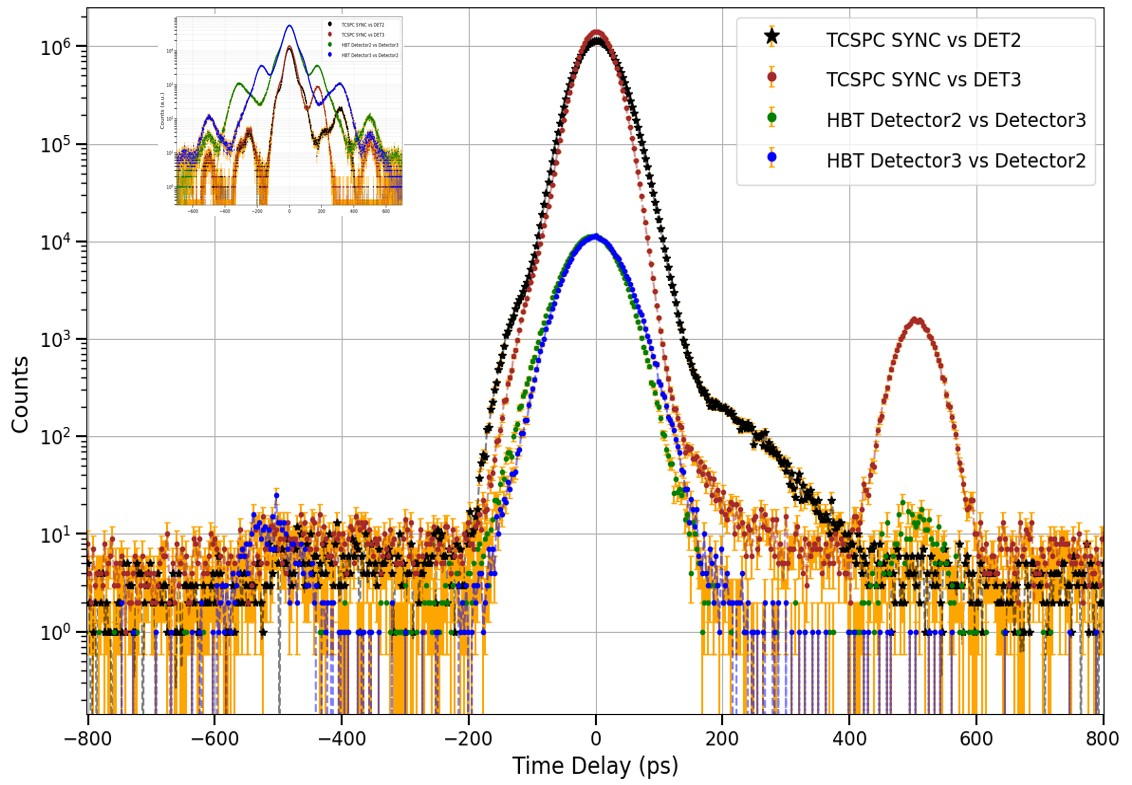
\includegraphics[width=1\textwidth]{CheckpointBravo_vs_Khaos.jpg}
\caption{Ciaone}
\label{RefinedMeasurement}
\end{figure}


% \subsection{Estimation of the width of the Detector response function}